\documentclass[aspectratio=169,11pt]{beamer}
\usepackage[utf8]{inputenc}
\usepackage[T1]{fontenc}
\usepackage[brazilian]{babel}
\usepackage{graphicx,array}
\usetheme{Singapore}

% Figuras independentes em figs/. Recompilar tudo: ./compilar.ps1
\definecolor{ink}{HTML}{202124}
\definecolor{muted}{HTML}{666666}
\definecolor{blue}{RGB}{30,80,160}
\definecolor{green}{RGB}{30,130,60}
\definecolor{red}{RGB}{190,60,60}
\definecolor{light}{HTML}{E8E8E8}
\setbeamercolor{normal text}{fg=ink,bg=white}
\setbeamercolor{structure}{fg=blue}
\setbeamersize{text margin left=8mm,text margin right=8mm}
\setbeamertemplate{navigation symbols}{}
\setbeamertemplate{footline}[frame number]
\newcommand{\bigtext}[1]{{\fontsize{24.88}{30}\selectfont #1\par}}

\title[Visitas domiciliares]{Planejamento de visitas domiciliares}
\subtitle{Rotas que consideram as regras do atendimento}
\author[Grupo C]{Luis Junior \and Manuela Dalmonte \and Vítor Feijó}
\date{INF99003 -- Ciclo 3 -- Grupo C\\Semana 1 | Pitch}
\hypersetup{pdfauthor={Luis Junior; Manuela Dalmonte; Vítor Feijó}}

\begin{document}

% 1 — Apresentar a base que será discutida, sem antecipar a inovação.
\begin{frame}[c]
  \titlepage
\end{frame}

\section{Problema}
% 2 — Ilustração conceitual, sem apresentar distância ou resultado inventado.
\begin{frame}{Uma rota precisa respeitar as prioridades}
  \vspace{5mm}
  \centering
  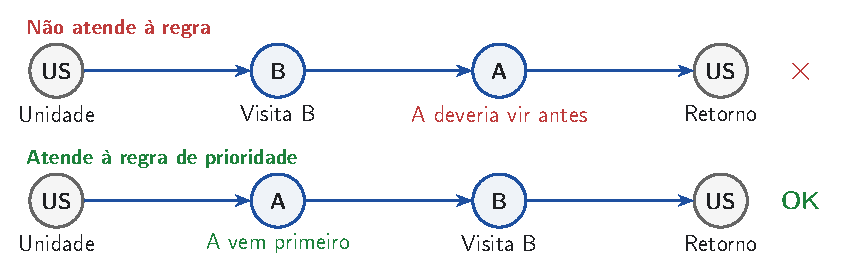
\includegraphics[width=\textwidth]{figs/01-rotas-e-regras.pdf}
\end{frame}

\section{Projeto-base}
% 3 — Restrições representadas no projeto, em linguagem operacional.
\begin{frame}{Regras e restrições do planejamento}
  \begin{columns}[T]
    \column{.30\textwidth}
    {\large\color{blue}Prioridades\par}
    \vspace{5mm}
    \centering
    Prioridade e atraso orientam a seleção e a ordem das visitas.
    \column{.30\textwidth}
    {\large\color{blue}Condições\par}
    \vspace{5mm}
    Habilitação, equipamento e assistência profissional necessários ao atendimento.
    \column{.30\textwidth}
    {\large\color{blue}Recursos\par}
    \vspace{5mm}
    Insumos e disponibilidade de assistência ao longo do turno.
  \end{columns}
  \vspace{7mm}
  {\large Uma decisão em uma visita pode afetar as seguintes.\par}
\end{frame}

% 4 — O roteirizador propõe a ordem; o planejador verifica ações/recursos.
\begin{frame}{Construção do plano de visitas}
  \centering
  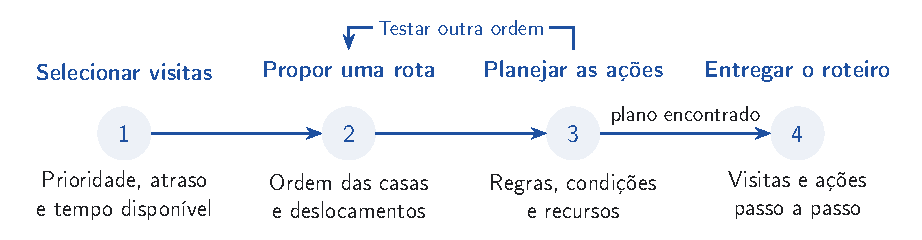
\includegraphics[width=\textwidth]{figs/02-planejamento-com-regras.pdf}
  \vspace{20mm}
  {\large\parbox{\textwidth}{\centering O resultado combina a ordem das visitas\\e as ações necessárias em cada parada.}\par}
\end{frame}

\section{Na prática}
% 5 — Exemplo didático de consumo e reposição, baseado nas ações do modelo.
\begin{frame}{A reposição de material faz parte do plano}
  \centering
  {\large Três visitas, uma unidade de material consumida em cada uma.\par}
  \vspace{6mm}
  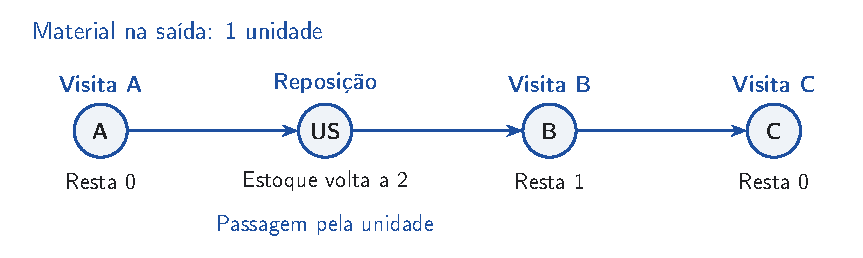
\includegraphics[width=\textwidth]{figs/03-reposicao-no-plano.pdf}
  \vspace{6mm}
  {\large\parbox{\textwidth}{\centering O planejamento inclui a passagem pela unidade\\para viabilizar as próximas visitas.}\par}
\end{frame}

% 6 — Diagnósticos que já existem no projeto; não são propostas de inovação.
\begin{frame}{Nem todo impedimento se resolve com outra rota}
  \renewcommand{\arraystretch}{1.2}
  \begin{tabular}{@{}m{.43\textwidth}@{\hspace{8mm}}m{.49\textwidth}@{}}
    {\large\color{blue}Situação identificada} & {\large\color{blue}Consequência para o plano}\\[5mm]
    Visitas fora da ordem de prioridade & Testar outra sequência de visitas.\\[6mm]
    Falta de uma condição exigida para o atendimento & Trocar a ordem não supre essa condição.\\[6mm]
    Assistência disponível insuficiente para as visitas previstas & Rever recursos ou visitas com a equipe.
  \end{tabular}\par
\end{frame}

% 7 — Regras sintéticas do domínio estendido, sem apresentá-las como normas.
\begin{frame}{Novas regras passam a fazer parte do planejamento}
  {\large O grupo testou a inclusão de três regras hipotéticas:\par}
  \vspace{7mm}
  \begin{columns}[T]
    \column{.30\textwidth}
    {\large\color{blue}Higienização\par}
    \vspace{4mm}
    Consumo e reposição de solução alcoólica.
    \column{.30\textwidth}
    {\large\color{blue}Proteção\par}
    \vspace{4mm}
    Disponibilidade de máscaras para visitas sinalizadas.
    \column{.30\textwidth}
    {\large\color{blue}Descarte\par}
    \vspace{4mm}
    Capacidade do coletor e troca na unidade.
  \end{columns}
  \vspace{9mm}
  {\large As novas condições foram consideradas\\sem alterar o mecanismo de busca.\par}
\end{frame}

% 8 — Valores e exemplo extraídos da saída já salva pelo Grupo B.
\begin{frame}{O resultado é um roteiro de trabalho}
  \begin{columns}[T,onlytextwidth]
    \column{.41\textwidth}
    {\large\color{blue}Exemplo simulado do projeto\par}
    \vspace{5mm}
    {\Large 6 visitas\par}
    \vspace{3mm}
    266 minutos estimados\par
    240 minutos disponíveis\par
    \vspace{4mm}
    {\large\color{red}Alerta: 26 minutos a mais\par}
    \column{.53\textwidth}
    {\large\color{blue}Trecho resumido do roteiro\par}
    \vspace{5mm}
    \textbf{Parada 2 -- Paciente 03}\par
    \vspace{4mm}
    Passar na unidade antes da visita para repor material.\par
    \vspace{5mm}
    Lista de tarefas por atendimento\par
    \vspace{3mm}
    Registro da visita no sistema
  \end{columns}
  \vspace{8mm}
  {\large A equipe recebe a sequência, as tarefas e os alertas do turno.\par}
\end{frame}

% 9 — Autoria do projeto original e responsabilidade pelo ciclo atual.
\begin{frame}{Encerramento e créditos}
  \centering
  {\large Obrigado pela participação!\par}
  \vspace{9mm}
  \begin{columns}[T,onlytextwidth]
    \column{.48\textwidth}
    \centering
    {\large\color{blue}Projeto original\par}
    \vspace{2mm}
    \textbf{Grupo B -- Ciclo 2}\par
    \vspace{4mm}
    Gabriel Knopp\par
    Arthur Silva\par
    Izadora Oliveira
    \column{.48\textwidth}
    \centering
    {\large\color{blue}Apresentação e próximo ciclo\par}
    \vspace{2mm}
    \textbf{Grupo C -- Ciclo 3}\par
    \vspace{4mm}
    Luis Junior\par
    Manuela Dalmonte\par
    Vítor Feijó
  \end{columns}
\end{frame}

\end{document}
